\documentclass[12pt,a4paper,twoside]{article}

%------------------------------ encoding
\usepackage[utf8]{inputenc}

%------------------------------ page layout
\usepackage[left=3cm,right=3cm,top=3cm,bottom=2cm]{geometry}

%------------------------------ clickable toc and links styles
\usepackage{hyperref}
\hypersetup{
    colorlinks,
    citecolor=black,
    filecolor=black,
    linkcolor=black,
    urlcolor=black
}

%------------------------------ font macro
\newcommand*{\courierfont}{\fontfamily{pcr}\selectfont}

%------------------------------ references
\usepackage{biblatex}
\addbibresource{bib.bib}

%------------------------------ tables
\usepackage{tabularx}

%------------------------------ images
\usepackage{graphicx}

%------------------------------ font preferences (1) or sc
\usepackage[sc]{mathpazo} 
% \usepackage{newpxmath}

%------------------------------ comment
\usepackage{comment}

%------------------------------ title spec
\usepackage{titlesec}
\usepackage{afterpage}

%------------------------------ abstract
\usepackage{abstract}
\renewcommand{\abstractnamefont}{\normalfont\Large\bfseries}

\begin{document}

\begin{comment}
\begin{titlepage}
    \centering
    \vspace*{\fill}

    \vspace*{0.5cm}
    
    \huge ACULEI
    
    \vspace*{2.5cm}
    
    \vspace*{1cm}

    \begin{minipage}{\textwidth}
        \centering
        \begin{tabular}{ccc}
            \small \textbf{Brajucha Filippo} & \small \textbf{Dinelli Michele} & \\
            \small University of Bologna & \small University of Bologna & \\
            \scriptsize \courierfont{\href{mailto:filippo.brajucha@studio.unibo.it}{filippo.brajucha@studio.unibo.it}} & \scriptsize \courierfont{\href{mailto:michele.dinelli5@studio.unibo.it}{michele.dinelli5@studio.unibo.it}} & \\
        \end{tabular}
    \end{minipage}

    \vspace*{1cm}

    \begin{minipage}{\textwidth}
        \centering
        \begin{tabular}{ccc}
            \small \textbf{Hanna Youssef} \\
            \small University of Bologna \\
            \scriptsize \courierfont{\href{mailto:youssefawni.hanna@studio.unibo.it}{youssefawni.hanna@studio.unibo.it}} \\
        \end{tabular}
    \end{minipage}
    
    \vspace*{\fill}
\end{titlepage}

\tableofcontents

\newpage

\end{comment}

\begin{center}

\rule[0.1cm]{15.8cm}{1.5mm}
{{\Large{Aculei}}} 
\rule[0.1cm]{15.8cm}{0.1mm}

\vspace*{1cm}

\begin{minipage}{\textwidth}
    \begin{tabular}{ccc}
        \small \textbf{Brajucha Filippo} & \small \textbf{Dinelli Michele} & \small \textbf{Hanna Youssef} \\
        \small University of Bologna & \small University of Bologna & \small University of Bologna \\
        \scriptsize \texttt{\href{mailto:filippo.brajucha@studio.unibo.it}{filippo.brajucha@studio.unibo.it}} & \scriptsize \texttt{\href{mailto:michele.dinelli5@studio.unibo.it}{michele.dinelli5@studio.unibo.it}} & \scriptsize \texttt{\href{mailto:youssefawni.hanna@studio.unibo.it}{youssefawni.hanna@studio.unibo.it}} \\
    \end{tabular}
\end{minipage}

\vspace*{1cm}
    
\end{center}

\begin{abstract}    
\noindent Questo report descrive le varie fasi del processo di realizzazione di un dataset che raccoglie i dati di fotografie di animali scattate automaticamente da foto-trappole situate nei boschi dell’Umbria. Realizzare il dataset ha lo scopo di raccogliere una vasta quantità di dati, così da metterli al servizio di tecniche di intelligenza artificiale, al fine di raggruppare e potenzialmente classificare le fotografie. \\ Si esplorano due approcci: il primo prevede l’apprendimento non supervisionato basato su algoritmi di clusterizzazione, il secondo si basa invece sull’utilizzo di una tecnica chiamata \textit{zero-shot image classification} al fine di classificare le fotografie in base all’animale ritratto. \\ Negli ultimi anni la disciplina nota come computer vision ha fatto passi enormi, grazie a questa branchia dell’informatica è possibile manipolare dati complessi, come le fotografie, estraendo da esse conoscenza. Le informazioni ottenute dalle fotografie, le relazioni e i pattern nascosti che vengono identificati dall'intelligenza artificiale sono utilizzati per generare un’esperienza interattiva all’interno di un archivio fotografico chiamato \textit{aculei}.
Il progetto \textit{aculei} nasce dall’idea di un fotografo milanese che ha posizionato varie foto-trappole automatiche nei boschi che circondano la casa in cui è cresciuto in Umbria. La volontà di pubblicare le fotografie e rendere l’esperienza sull’archivio ai-driven sono le motivazioni che lo spingono a ideare il progetto \textit{aculei}.
\end{abstract}

\section{Introduzione}
La computer vision è un campo dell'intelligenza artificiale che permette ai computer di estrarre informazioni e dati da immagini digitali, video e altri input visivi. Funziona più o meno come la vista umana, ma gli umani hanno un grande vantaggio: dispongono di anni e anni di esperienza in cui si sono allenati a distinguere gli oggetti \cite{ibm-comp-vision}. I computer devono fare lo stesso ma in molto meno tempo ricorrendo generalmente a tecniche di deep learning sfruttando una tipologia di reti neurali note come reti neurali convoluzionali. Sono state utilizzate diverse tecniche basate sulla computer vision come ocr \footnote{Ocr: optical character recognition è un termine che descrive i programmi dedicati al riconoscimento ottico dei caratteri in un documento} e zero-shot image classification \footnote{Task di computer vision per la classificazione di immagini in una determinata classe, senza alcun addestramento o conoscenza preventiva delle classi}. \\ Per realizzare il dataset di aculei è stata ampiamente sfruttata la computer vision in quanto i dati forniti sono più di 16000 immagini digitali che devono essere necessariamente processate da un computer.

\begin{figure}[!ht]
    \centering
    \includegraphics[width=\textwidth ,height=\textheight, keepaspectratio]{assets/TF_ACULEI_16567_DSCF0121.jpg}
    \caption{Esempio di immagine digitale scattata da una delle foto-trappole}
    \label{fig:enter-label}
\end{figure}

\subsection{Descrizione del Problema}
Si vuole creare un dataset contenente i dati di fotografie scattate automaticamente da foto-trappole 
posizionate in Umbria. Le fotografie sono state rese disponibili dal fotografo proprietario delle foto-trappole che le ha raccolte negli ultimi 4 anni. \\ Dalle fotografie si vogliono estrarre i dati principali quali la temperatura, la fase lunare, la camera che ha scattato l'immagine, la data e l'ora. Molto ambizioso è il riconoscimento dell'animale ritratto. Le fotografie possono contenere tra i meta-dati alcune di queste informazioni mentre alcune volte sono del tutto assenti come ad esempio la misurazione della temperature e le informazioni sulla tipologia di animale. La perdita di alcune informazioni nei meta-dati potrebbe essere causata da software intermedi che ha utilizzato il fotografo per processare le foto prima di fornirle per lo studio. \\ Il problema quindi è definire una serie di procedure per processare le immagini, estraendo da esse le informazioni rilevanti e quindi creare un dataset sul quale applicare tecniche di intelligenza artificiale per identificare correlazioni tra le fotografie così da offrire un'esperienza coinvolgente sull'archivio fotografico che le raccoglie.

\subsubsection{Motivazione del problema e rilevanza}
Il progetto aculei nasce dalla volontà del fotografo proprietario delle foto-trappole di rendere pubbliche le fotografie sviluppando un archivio fotografico online con forte impronta artistica. Oltre agli studi stilistici legati all'interazione e all'esperienza utente è stato previsto uno studio applicando l'intelligenza artificiale così che sia essa a guidare l'esperienza utente sull'archivio. Nel contesto del progetto aculei la fase descritta in questo documento rappresenta un punto molto importante per lo sviluppo del sistema di backend legato all'archivio fotografico.

\subsubsection{Pubblico interessato}
Le persone interessate a questo progetto sono coloro che vogliono osservare le varie fasi di creazione di un dataset a partire dalla raccolta dei dati fino alla realizzazione del dataset completo. Inoltre potrebbero essere interessati anche coloro che vogliono utilizzare il dataset per studi propri o ampliare e migliorare quelli al momenti svolti.

\begin{comment}
\subsubsection{Benefici di una soluzione}
Definire gli step necessari alla creazione del dataset e realizzarlo significa completare la componente che gestisce l'interazione sull'archivio \textit{aculei}. 
\end{comment}

\subsection{Soluzione Proposta}

\subsubsection{Approccio alla soluzione}
Per arrivare alla soluzione abbiamo eseguito diversi tenativi con molteplici tecnologie, più o meno 
sofisticate, che ci hanno restituito sia ottimi risultati che pessimi.\\
Per ottenere la soluzione ottima a cui siamo arrivati abbiamo attraversato un percorso con molti ostacoli, 
è stato fondamentale mantere la comunicazione nel gruppo. Molto spesso ci siamo trovati a discutere su 
strade alternative o possibili soluzione a problemi, sicuramente senza la discussione tra di noi non 
saremmo mai arrivati ad una conclusione rapidamente e avremmo impiegato molto più tempo ad affrontare le 
insidie.\\
La prima soluzione a cui avevamo pensato è stata quella di addestrare un AI con diverse immagini per poi 
cercare di ottenere un output soddisfacente ed efficiente in cui essa avrebbe dovuto riconoscere lo stesso 
animale presente nella foto. Il processo è stato piuttosto complesso e vedendo gli scarsi risultati abbiamo 
abbandonato quasi subito questa idea.\\
Dopo aver ottenuto dei risultati poco soddisfacenti ci siamo riuniti con il Professore per cercare di 
trovare insieme una soluzione più congeniale, lui ci ha aiutato molto nell'esplorare altre idee pensando un 
po fuori dagli schemi, osservando il problema da fuori e ri-organizzando il materiale a disposizione in 
modo da lavorare con maggiore chiarezza e professionalità.\\
Abbiamo quindi deciso di proseguire per un'altra soluzione altrettanto valida e, probabilmente, più adeguata 
alla risoluzione del nostro problema. La scelta è stata quella di eseguire una clusterizzazione sulle 
immagini in modo da creare dei \textit{pool} di immagini correlate, cambia quindi l'idea iniziale di 
riconoscere l'animale ma viene mantenuta l'idea di un percorso interattivo ed espositivo.\\
Durante la realizzazione di questa soluzione abbiamo approfondito l'uso di diversi algoritmi di clustering 
e il tuning degli stessi, modificando parametri, numero di clusters, tipologie di dati ecc.
\subsubsection{Sfide informatiche affrontate}
I problemi sono stati molteplici e si sono distribuiti uniformemente durante tutta la realizzazione del 
progetto. Ne abbiamo riscontrati sia durante la prima fase in cui abbiamo cercato di allenare l'AI che 
durante la preprazione del dataset per la clusterizzazione.\\
Inizialemente il problema principale è stato quello di avere delle immagini chiare e simili in modo da 
poter insegnare quali fossero i tratti caratterstici di ciascun animale, ma essi risultavano troppo 
confusionarie e poco equiparabili, alcune erano sfocate, altre tagliate, altre ancora super luminose e 
altre totalmente buie. Un altro problema durante questa fase è stato quello della dimensione delle foto, 
esse risultavano troppo pesanti e dettagliate, quindi ingestibili dalla potenza di calcolo delle macchine 
che abbiamo a disposizione.\\
I problemi sono proseguiti nella fase della clusterizzazione, uno dei lavori più lunghi e macchinosi è 
stato quello di realizzare il dataset. Abbiamo docuto scegliere quale features tenere, quali fossero le 
più interessanti e quelle più facilmente reperibili in modo da avere pochi valori \textit{null}. Una volta 
scelti i valori da studiare abbiamo dovuto capire quale fosse il metodo migliore per ottenerli, abbiamo 
provato diverse tipologie di strumenti e diverse versioni degli stessi (molteplici OCR e diversi lettori 
di filesystem).\\
Infine abbiamo riolto diversi problemi legati alla memorizzazione dei dati in modo corretto, nonostante 
le diverse tecniche testate abbiamo avuto diversi problemi di dati inconsistenti e quindi abbiamo dovuto 
risolvere molti problemi di valori \textit{null} all'interno del dataset. Talvolta abbiamo dovuto anche 
calcolare dei dati in modo da avere più informazioni da analizzare (come le stagioni o le fasi lunari), 
oppure convertirne alcuni in mdo da renderli sensati dal punto di vista della clusterizzazione (con dei 
one-hot-encoder ad esempio).\\
Nonostante queste accortezze non siamo comunque riusciti a creare un dataset con tutti i dati che volevamo 
ma comunque alcuni sono andati persi.
\subsubsection{Rassegna della letteratura}
\textit{DA ESTENDERE}
\subsubsection{Divisione dei compiti nel gruppo}
Il gruppo ha lavorato abbastanza uniformemente nella realizzazione del progetto, tutti hanno partecipato 
in modo differente al completamento dello stesso.\\
Durante la stesura del codice è risultato fondamentale un approccio in cui ognuno fosse libero di 
criticare e consigliare quale fosse la soluzione ideale per lui. Ci sono state molte situazioni in cui 
ci siamo riuniti e abbiamo provato ad ideare e sviluppare delle idee per poter risolvere i problemi 
incontrati nel percorso.\\
\textit{DA ESTENDERE}
\subsubsection{Risultati ottenuti in sintesi}
\textit{DA ESTENDERE}


\newpage
\section{Metodo Proposto}

\subsection{Scelta della Soluzione}
La soluzione scelta è stata quella di creare un percorso interattivo tra immagini correlate in 
grado di coinvolgere e stupire l'utente in modo dinamico. Questa soluzione è stata ottenuta 
eseguendo una clusterizzazione della raccolta di immagini.\\
Una volta raccolte tutte le fotografie, sono state categorizzate e indicizzate in modo da creare 
un dataset di informazioni, da studiare e ordinare per poi proporre un percorso interessante 
all'utente finale.\\
Le soluzioni proposte non sono state poche, abbiamo provato diversi metodi e testato diverse 
tecnologie per ottenere il risultato migliore, quello che coincidesse esattamente con le nostre 
necessità di avere un sistema reattivo e sempre pronto ad essere aggiornato e migliorato con 
altre immagini e informazioni, personalizzabile dall'utente e utile sia come intrattenimento, 
quindi a scopo ludico, che interessante dal punto di vista scientifico e dell'osservazione. Per 
questo abbiamo studiato e ci siamo anche informati su quali potessero essere le correlazioni 
scientifiche con ciò che osservavamo e ciò che valutavamo, in modo da poter avere anche un 
occhio critico per poter valutare se i risultati scovati fossere corretti oppure inutili e 
sbagliati. Non essendo una materia di nostra competenza, infatti, abbiamo dovuto prestare molta 
attenzione.\\
La soluzione corretta è stata scelta anche dopo aver effettuato dell'inferenza sui dati in modo 
da osservare la distribuzione degli stessi e capire se ci fossero stati dei problemi. 
\subsubsection{Alternativi considerati e giustificazioni della scelta}
Inizialmente abbiamo provato a realizzare un'AI in grado di riconoscere l'animale selvatico 
dall'immagine, una sorta di \textit{lens} in grado di analizzare la foto e il contesto per poter 
tracciare quale fosse il soggetto della foto. L'idea è stata abbandonata piuttosto velocemente 
perchè le risorse a disposizione erano molto inferiori a quelle richieste da un lavoro così 
costoso computazionalmente parlando.\\
Per questo abbiamo optato per una soluzione più alla nostra portata e ugualmente molto 
interessante, abbiamo creato un dataset con le immagini a nostra disposizione abbiamo provato 
ad utilizzare diversi metodi di clusterizzazione con diverse features da considerare e diverso 
numero di clusters.\\
Dopo diverse prove e ricerche abbiamo capito che solo empiricamente e provando si può ottenere 
il risultato migliore e più adatto alle esigenze, seguendo anche delle regole teoriche come ad 
esempio l'\textbf{Elbow Method}, un metodo euristico che aiuta a scegliere il numero di 
clusters necessari per ottenere il risultato migliori in termini di scelte di features e numero 
di clusters.\\
\subsubsection{Metodologia per la misurazione delle performance}
La misurazione della performance è avvenuta tramite diversi metodi e in diversi momenti durante la 
realizzazione di questo progetto. Abbiamo sempre cercato di ottenere dei buoni risultati tenendo 
sotto controllo i dati ottenuti.\\
Per questo motivo, durante la creazione del dataset, abbiamo effettuato diversi test e diverse 
misurazioni per vedere se i dati in output fossero sensati e collezionati nel modo corretto senza 
particolari incongruenze.\\
Per il nostro progetto risulta molto complesso parlare di misurazione della performance visto che 
il risultato proposto è soggettivamente buono e non può essere valutato da parametri numerici. 
Generalmente possiamo osservare che i risultati proposti sono di nostro gradimento ma sicuramente 
possono esserci delle personalizzazioni che magari cambiano l'output in modo da ottenerne uno più 
utile al proprio scopo, magari modificando le varibaili della clusterizzazione o il numero di 
clusters.

\section{Risultati Sperimentali}

\subsection{Dimostrazione e Tecnologie}
\subsubsection{Istruzione per la dimostrazione}
La dimostrazione che si ottiene non è altro che un percorso tra delle immagini che sono 
evidentemente correlate, secondo le features che abbiamo deciso di inserire nella clusterizzazione, 
ovvero: \textit{[Inserire le features scelte per la clusterizzazione]}.
\subsubsection{Tecnologie e versioni usate (riproducibilità)}
Le immagini sono state scattate e raccolte maualmente da alcune foto-trappole, convertite poi in 
formato \texttt{.jpeg} e caricate su dropbox, tramite il quale è stato possibile lavorare senza 
avere con se la copia fisica delle imamgini stesse.\\ 
Per gli l'algoritmo di clustering è stato utilizzato Python con alcune sue librerie per poter 
gestire e raccogliere i dati.\\
\textit{DA ESTENDERE} 

\subsection{Risultati}

\setlength{\tabcolsep}{0.5em} % horizontal padding
{\renewcommand{\arraystretch}{1.5} % vertical padding
    \begin{tabular}{|l|l|l|l|l|}
        \hline
        \textbf{image\_name} & \textbf{camera} & \textbf{date\_time} & \textbf{moon\_phase} & \textbf{temperature} \\ 
        \hline
        a & b & c & d & f\\
        \hline
    \end{tabular}
}

\begin{figure}[h!]
    \centering
    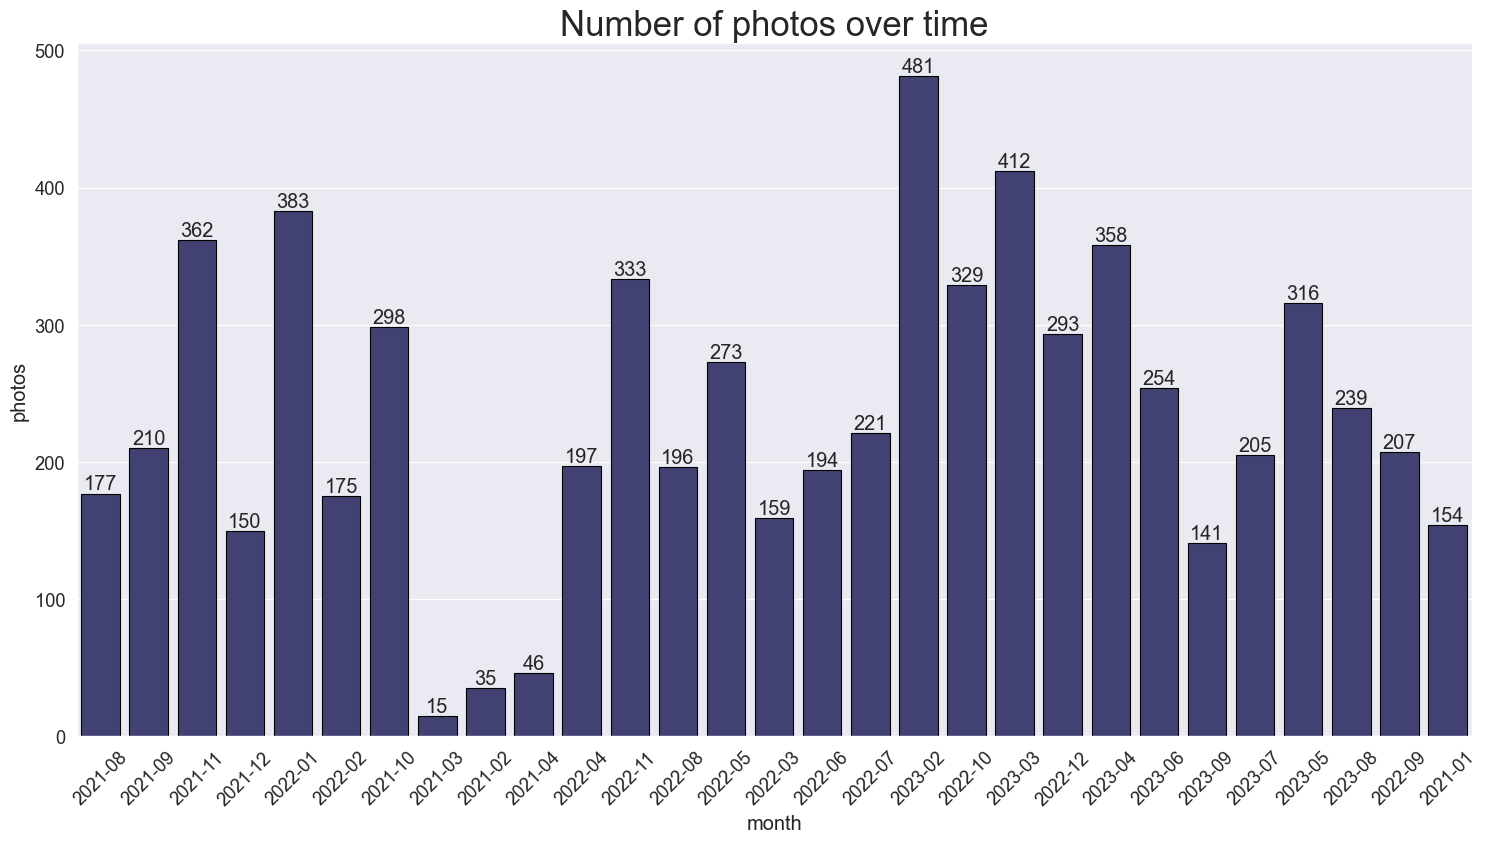
\includegraphics[width=\textwidth ,height=\textheight, keepaspectratio]{assets/photos-ot.png}
    \caption{Numero totale di fotografie per ogni mese}
    \label{fig:photos-ot}
\end{figure}

\begin{figure}[h!]
    \centering
    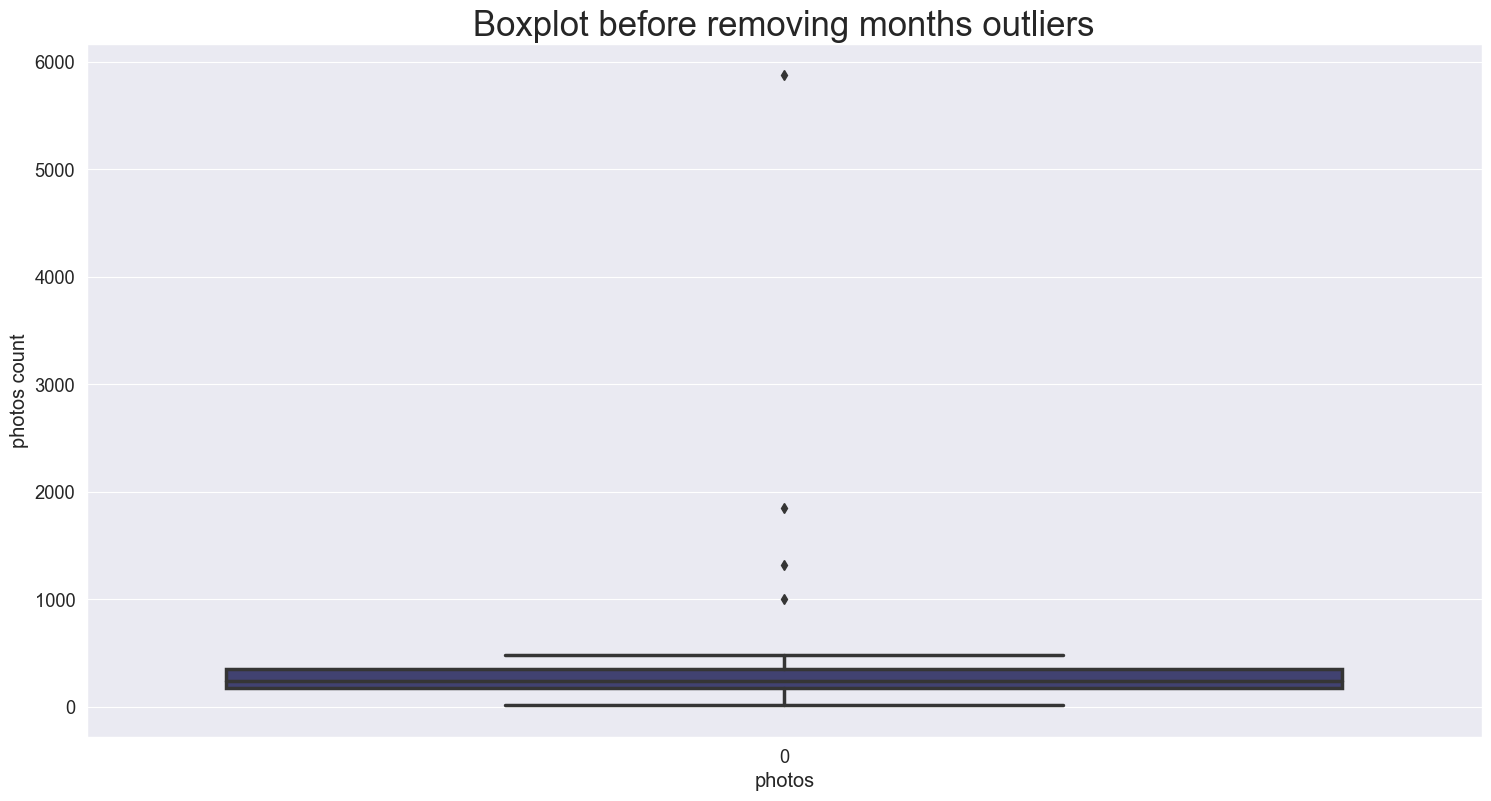
\includegraphics[width=\textwidth ,height=\textheight, keepaspectratio]{assets/boxplot-outliers.png}
    \caption{Boxplot dei dati prima di rimuovere gli outliers}
    \label{fig:boxplot-outliers}
\end{figure}

\begin{figure}[h!]
    \centering
    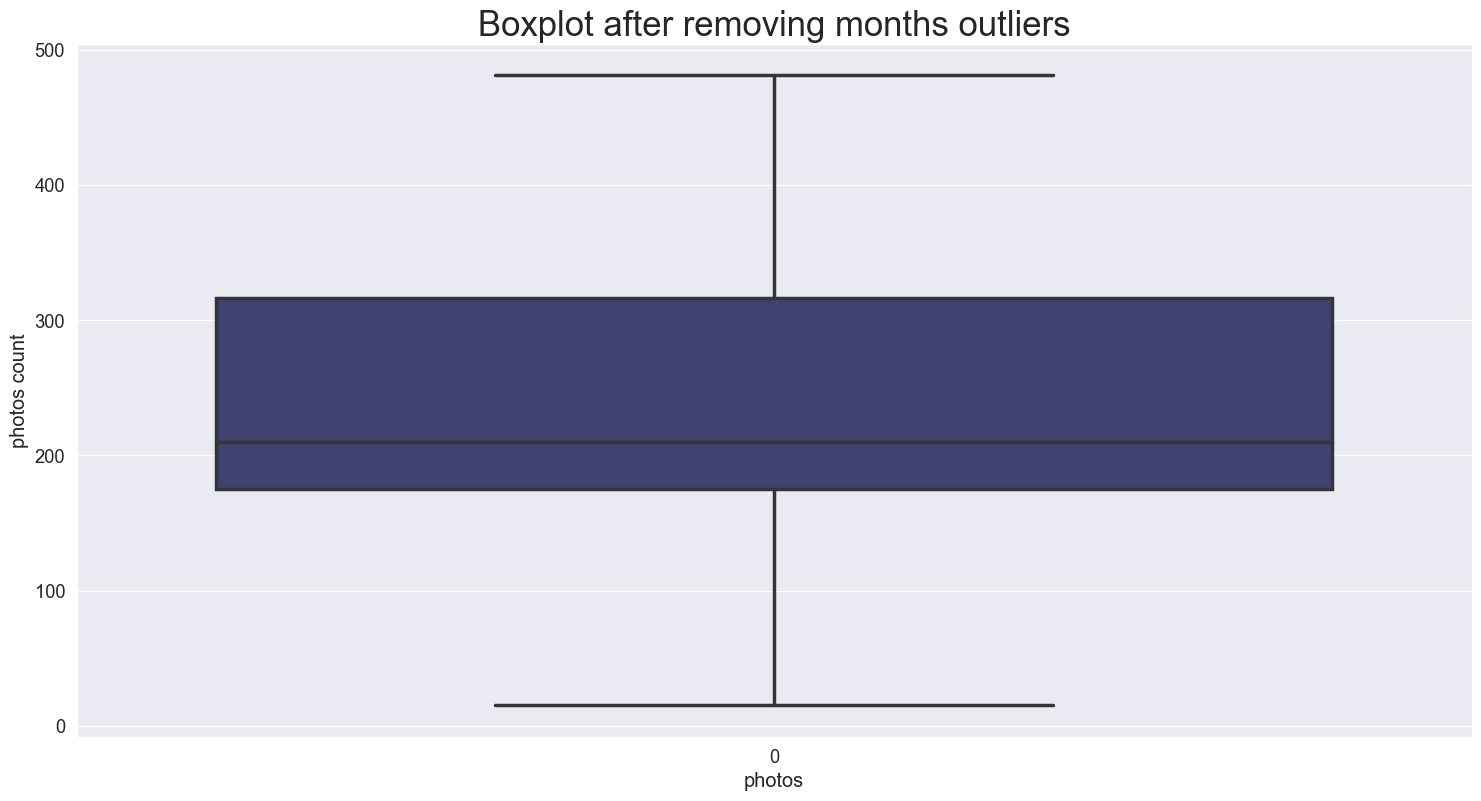
\includegraphics[width=\textwidth ,height=\textheight, keepaspectratio]{assets/boxplot-wout-outliers.png}
    \caption{Boxplot dei dati dopo aver rimosso gli outliers}
    \label{fig:boxplot-wout-outliers}
\end{figure}


\subsubsection{Risultati della configurazione migliore}
\subsubsection{Studio di ablazione: confronto tra configurazioni}
\subsubsection{Studio di comparazione con letteratura}


\newpage
\section{Discussione e Conclusioni}

\subsection{Discussione dei Risultati}
\subsubsection{Analisi delle performance rispetto alle aspettative}

\subsection{Validità del Metodo}
\subsubsection{Valutazione se il metodo rispetta le aspettative}

\subsection{Limitazione e Maturità}
\subsubsection{Limiti di applicabilità e bias}

\subsection{Lavori Futuri}
\subsubsection{Proposte per avanzare il progetto}

\newpage

\printbibliography

\end{document}